\documentclass[conference,a4paper]{IEEEtran}
\IEEEoverridecommandlockouts
% The preceding line is only needed to identify funding in the first footnote. If that is unneeded, please comment it out.
\usepackage{cite}
\usepackage{amsmath,amssymb,amsfonts}
\usepackage{algorithmic}
\usepackage{algorithm}
\usepackage{graphicx}
\usepackage{textcomp}
\usepackage{multirow}
\usepackage{booktabs}
\usepackage{color}
\usepackage[T1]{fontenc}
\usepackage[table,xcdraw]{xcolor}
\def\BibTeX{{\rm B\kern-.05em{\sc i\kern-.025em b}\kern-.08em
T\kern-.1667em\lower.7ex\hbox{E}\kern-.125emX}}
\begin{document}

\title{Reference Model of Middle Homework 1
}


\author{\IEEEauthorblockN{Ruike Lyu$^{1}$}
\IEEEauthorblockA{Department of Electrical Engineering, Tsinghua University, Beijing, China$^{1}$}
\IEEEauthorblockA{Email: lvruike1999@163.com$^{1}$}

% \thanks{This work was supported by the Major Smart Grid Joint Project of the National Natural Science Foundation of China and State Grid under Grant U2066205 and National Natural Science Foundation of China under Grant 52107102}

}

\maketitle

\section{Background}

We focus on secondary frequency regulation, also known as automatic generation control. Secondary frequency regulation is a process designed to maintain the system frequency close to a nominal value by correcting  frequency and power mismatches that persist after primary regulation. Compared to primary regulation, secondary frequency regulation typically has a slower response, taking place over a period of a few seconds to several minutes, making it suitable for the participation of demand-side resources.

We assume that the VPP can conveniently obtain the cost characteristics, operating parameters, and states of its internal resources based on which it formulates the bidding strategy and controls their power consumption/production. Because of the relatively small capacity of the resources, we regard the VPP as a price taker that jointly optimizes its bids for energy (baseline power) and regulation capacity in the market, with the forecast market prices as the boundary condition. 

Before actually providing frequency regulation, the VPP  receives its accepted regulation capacity $r$ after market clearing, which should be consistent with its bids since a price taker can declare a regulation capacity with a minimum price to guarantee acceptance. When actually providing frequency regulation (known as regulation deployment), the GO sends regulation signals $\delta \in [-1, 1]$  to the VPP (e.g., every 2 seconds in PJM). The product of the regulation signal and the regulation capacity $\delta r$ is the to-be-adjusted output of the VPP. 

\section{Model Formulation}\label{sec_method}

The virtual battery (VB) model describes the operation of DERs using time-coupled power and energy constraints, which can be applied to model common resources such as energy storages, electric vehicles and thermostatically controlled loads. We employ the VB model to formulate the coupled energy-regulation constraints of the DERs. For resource $i$, its hourly output needs to satisfy the operation constraints for power limits (\ref{model_energy_powerLimit}), energy limits (\ref{model_energy_energyLimit}), change of energy (\ref{model_std_energyChange}), and initial energy (\ref{model_energy_energyInit}):
\begin{subequations}\label{model_energy}
  \begin{equation}\label{model_energy_powerLimit}
    0 \le p^{\rm dis(ch)}_{t, i} \le \overline{p}^{\rm dis(ch)}_{t, i} \ : \ \underline{\mu}^{\rm pd(c)}_{t, i}, \overline{\mu}^{\rm pd(c)}_{t, i}, \ \forall  t
  \end{equation}\vspace{-0ex}
  \begin{equation}\label{model_energy_energyLimit}
    \underline{e}_{t, i} \le e_{t, i} \le \overline{e}_{t, i} \ : \ \underline{\mu}^{\rm e}_{t, i}, \overline{\mu}^{\rm e}_{t, i},\ \forall t
  \end{equation}\vspace{-0ex}
  \begin{align}\label{model_std_energyChange}
    e_{t+1, i} = & e_{t, i} + 
    (\eta^{\rm ch} p^{\rm ch}_{t, i} -  \frac{1}{\eta^{\rm dis}} p^{\rm dis}_{t, i}) \Delta t \ : \ \lambda^{\rm e}_{t, i},\ \forall t
  \end{align}\vspace{-0ex}
  \begin{equation}\label{model_energy_energyInit}
    e_{t, i} = e_{0, i} \ : \ \lambda^{\rm e0}_{i},\ t = 1
  \end{equation}
\end{subequations}
where $p_{t, i}$ and $r_{t, i}$ represent the output and regulation capacity for time interval $t$; $e_{t, i}$ is the energy at the beginning of $t$; the underlined/overlined parameters represents the lower/upper limit of the corresponding variables; the superscript dis(d)/ch(c) represent discharging to/charging from the grid; $e_{0, i}$ is the initial energy. $\eta$ is the (dis)charging efficiency. $\mu$ and $\lambda$ are the Lagrangian multipliers of the corresponding constraints, which won't be used here, so you can ignore them.

The constraints for resource $i$ providing regulation include non-negative capacity (\ref{model_reg_nonnegative}), power capacity limits (\ref{model_reg_powerLimit1}-\ref{model_reg_powerLimit2}), and maintenance time requirements (\ref{model_reg_req1}-\ref{model_reg_req2}):
\begin{subequations}\label{model_reg}
  \begin{equation}\label{model_reg_nonnegative}
    r_{t, i} \ge 0 \ : \ \underline{\mu}^{r}_{t, i}, \ \forall t
 \end{equation}\vspace{-0ex}
 \begin{equation}\label{model_reg_powerLimit1}
  p^{\rm dis}_{t, i} - p^{\rm ch}_{t, i} + r_{t, i} - \overline{p}^{\rm dis}_{t, i} \le 0 
  \ : \ \mu^{rpd}_{t, i}, \ \forall t
\end{equation}\vspace{-0ex}
\begin{equation}\label{model_reg_powerLimit2}
  - p^{\rm dis}_{t, i} + p^{\rm ch}_{t, i} + r_{t, i} - \overline{p}^{\rm ch}_{t, i} \le 0
  \ : \ \mu^{rpc}_{t, i}, \ \forall t
\end{equation}\vspace{-0ex}
\begin{equation}\label{model_reg_req1}
    \eta^{\rm ch} (r_{t, i} - p^{\rm dis}_{t, i} + p^{\rm ch}_{t, i}) \Delta t^{req} + e_{t, i} - \overline{e}_{t, i} \le 0
    \ : \ \mu^{rec}_{t, i}, \ \forall t
 \end{equation}\vspace{-0ex}
  \begin{equation}\label{model_reg_req2}
    \frac{1}{\eta^{\rm dis}} (r_{t, i} + p^{\rm dis}_{t, i} - p^{\rm ch}_{t, i}) \Delta t^{req} - e_{t, i} + \underline{e}_{t, i} \le 0
    \ : \ \mu^{red}_{t, i}, \ \forall t
\end{equation}
\end{subequations}
where $\Delta t^{req}$ represents the duration required for the resource to maintain its maximum regulation output, for example, 15 minutes in PJM~\cite{he_optimal_2016}. The bids of the VPP are the aggregated bids of the DERs, which are represented as:
\begin{equation}\label{model_vpp_aggBid}
  p_t = \sum_{i=1}^{I} (p^{\rm dis}_{t, i} - p^{\rm ch}_{t, i}), \ r_t = \sum_{i=1}^{I} r_{t, i}, \ \forall t
\end{equation}\vspace{-0ex}

In the above model, the parameters are $\theta = \{\overline{p}^{\rm dis(ch)}_{t, i}, \underline{e}_{t, i}, \overline{e}_{t, i}, e_{0, i}, \forall t \forall i\}$, and the internal variables are $y = \{p_{t, i}, r_{t, i}, e_{t, i}, \forall t \forall i\}$. The constraints $h(\cdot)$ are the combination of Equations (\ref{model_energy})-(\ref{model_vpp_aggBid}). 

 Thus, the joint energy-regulation bidding of the VPP is formulated as the optimization problem below:
\begin{subequations}\label{model_bid_primal}
\begin{equation}\label{model_vpp_profit}
    \underset{p_{[T]}, r_{[T]}}{\rm max.} \sum_{t=1}^{T}(Pr^{\rm e}_{t} p_{t} + Pr^{\rm r}_{t} r_{t} 
    - Pr^{\rm deg}(p_{t}))\Delta t
\end{equation}\vspace{-0ex}
\begin{equation}\label{model_vpp_constraint}
  {\rm s.t.} \ (\ref{model_energy})-(\ref{model_vpp_aggBid})
\end{equation}
\end{subequations}
where $T$ and $I$ represent the number of scheduling time intervals and DERs, respectively. The variables with subscript $[T]$ is a shorthand notation for a T-dimensional vector, for example, $p_{[T]} = (p_1, p_2, ..., p_T)$ and $r_{[T]} = (r_1, r_2, ..., r_T)$ represent the hourly (baseline energy) output and regulation capacity of the VPP, respectively; $Pr^{\rm e}_{t}$ is the energy price; $Pr^{\rm r}_{t} = s^{\rm perf} (Pr^{\rm cap}_{t} + Pr^{\rm mil}_{t} a^{\rm mil}_{t})$ is the equivalent regulation capacity price for the VPP; $s^{\rm perf}$ is the performance score, $Pr^{\rm cap(mil)}_{t}$ is the regulation capacity(mileage) price, and $a^{\rm mil}_{t}$ is the expected regulation mileage for $t$. $Pr^{\rm deg}$ is the cost function of the resources. We assume that $Pr^{\rm deg}$ is directly proportional to the total discharge power of the VPP.

Given the energy-regulation price $(Pr^{\rm e}_{[T]}, Pr^{\rm r}_{[T]})$, solving (\ref{model_bid_primal}) using the original VPP operation model can obtain the optimal bidding results $(p_{[T]}, r_{[T]})$.


\section{Model Parameters}\label{sec_numerical}

% Scenario
\begin{figure}[!t]
  \centering
    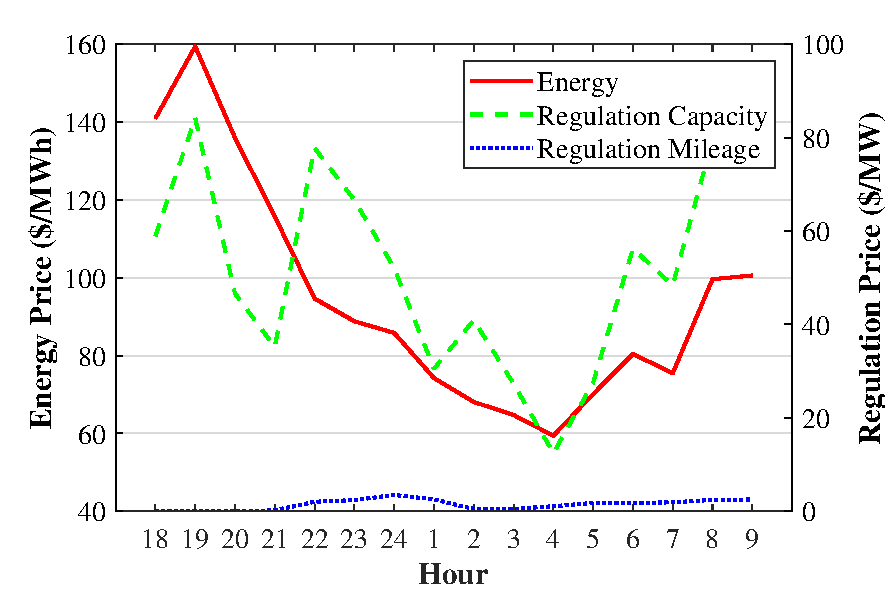
\includegraphics[width=1.5in]{figures/price.pdf}
    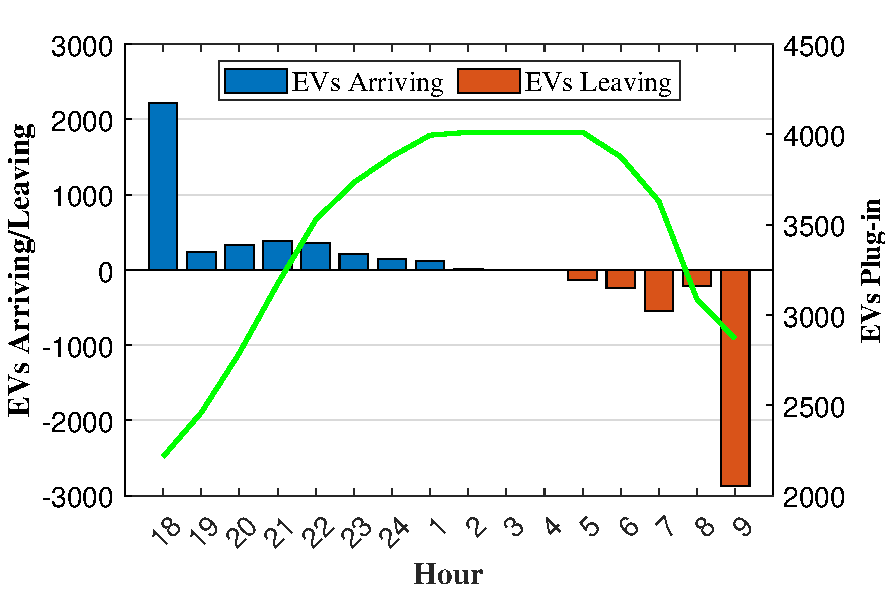
\includegraphics[width=1.5in]{figures/ev_arrive_leave.pdf}
\caption{Scenario setting: (left) typical energy / regulation prices of PJM (July 27, 2022). (right) The arriving / leaving time of the EVs.}
  \label{fig_scenario}
\end{figure}

We borrowed the scene of aggregating 4012 electric vehicles (EVs) for providing energy and regulation services from Ref.~\cite{lyu_co-optimizing_2023}. The EV batteries were charged starting from 0kWh using bidirectional 7.68kW charging piles, and it was required that the battery level at departure was not less than 80\% of the maximum capacity of 50kWh. The compensation for battery discharging was set at \$0.1/kWh. Readers can refer to Ref.~\cite{lyu_co-optimizing_2023} for detailed scenario setting. Other market parameters include the length of (scheduling) time interval $\Delta t = 1$ hour,
the required maintenance time $\Delta t^{\rm req} = 0.25$ hours, and
the performance score $s^{\rm perf} = 0.984$. The regulation mileage was estimated using historical data. Please note that we have given the calculated $Pr^{\rm r}_{[T]}$ in the attachment, so it does not need to be calculated with $a^{\rm mil}_{t}$.



\bibliographystyle{IEEEtran}
% argument is your BibTeX string definitions and bibliography database(s)
\bibliography{reference}

\end{document}
